\chapter{Разработка алгоритма}

Большинство алгоритмов сжатия обучают свою модель в процессе сжатия текста основываясь на только что полученных данных. 
Исходные данные, которые рассматриваются в нашей задаче, не позволяют так делать, так как данных
 одного сообщения зачастую слишком мало, чтобы заметить в них закономерности. Поэтому необходим алгоритм, 
 который может обучиться на полном наборе сообщений, а потом использовать полученные знания для кодирования 
 отдельных сообщений. При этом полученные знания должны быть сохранены достаточно компактно. 

\section{Однобуквенный Хаффман}
В качестве основы для нашего решения был взят алгоритм Хаффмана~\cite{huffman}, 
так как он позволяет заранее построить модель на исходных данных, а потом использовать ее для сжатия 
отдельных сообщений. Идея  алгоритма достаточно проста. Пусть у нас есть алфавит из $n$ символов. 
Посчитаем $cnt_i$~--- количество раз, которое символ $i$ встречается в исходном наборе сообщений.
 Положим $p_i = \frac{cnt_i}{\sum{cnt_i}}$~--- вероятность встретить символ $i$. Далее каждому символу $i$ ставится 
 в соответствие некоторая битовая строка $s_i$, такая что $\sum\limits_{i} |s_i| \cdot p_i$ как можно меньше и 
  $\forall i \neq j : s_i \text{ не является префиксом } s_j$. Второе условие позволяет однозначно декодировать закодированное
   сообщение, а первое говорит о том, что код является оптимальным среди всех префиксных кодов.
После того как получены строки $s_i$ можно приступать к кодированию. Для этого алгоритм рассматривает все
 символы строки слева направо и заменяет символ $i$ на битовую строку $s_i$.

Чтобы декодировать сообщение алгоритм рассматривает битовую запись полученных данных. Каждый раз
 выбирается строка $s_i$, которая является префиксом еще не декодированных данных, на выход записывается 
 символ $i$, а из исходных данных выкидываются первые $|s_i|$ символов. Заметим, что существует только 
 одна строка $s_i$, которая может быть взята, так как код является префиксным. Чтобы быстро осуществлять
  поиск подходящей строки $s_i$ все строки удобно добавить в структуру данных префиксное дерево \cite{knuth}.

Достоинством этого алгоритма является количество данных, которые ему нужно хранить после обучения 
на исходном наборе сообщений. А именно, единственное, что нужно знать алгоритму, это количество 
вхождений каждой буквы в сообщениях. Если считать, что размер алфавита $256$, а количество вхождений
 хранится в $32$-битном типе данных, то на хранение дополнительной информации потребуется всего $256\times 4 = 1024$ байт = $1$ кбайт.
К сожалению, эффективность сжатия у такого алгоритма не очень высокая. В частности на тестовой 
выборке сообщений был получен коэффициент сжатия 1,37.
 
\section{Хаффман по словам} 
Логичным улучшением этого подхода является изменение алфавита. А именно, в качестве алфавита
 можно использовать не $256$ символов, а, например, слова \cite{handbook}. 
 Предлагается поддерживать два отдельных словаря. Один для того, что называется словами в обычном
  понимании, а другой для знаков препинания и всего остального. При этом в сообщениях слова из
   двух словарей должны строго чередоваться. Также при кодировании необходимо указать из какого 
   словаря взято первое слово. Либо всегда считать, что оно из конкретного словаря, но тогда в 
   него необходимо добавить <<пустое>> слово и, соответственно, подсчитать его вероятность. 
Для разделения на слова и знаки пунктуации будем использовать следующий метод. Разделим все символы, 
которые могут встречаться, на два множества. В первое отнесем большие и маленькие буквы
 (как латинские, так и кириллические), а во второе все остальные. Словом будем считать наибольший 
 по включению набор соседних символов, которые лежат в одном множестве. 

В \cite{handbook} отмечены следующие недостатки данного метода:
\begin{enumerate}
	\item словари достаточно большие. Поэтому они могут не помещаться в память, и для работы с ними нужно 
использовать эффективные алгоритмы;
	\item на входных данных маленького размера практически все слова различны и поэтому алгоритм не успеет 
обучиться;
	\item необходимо два прохода по данным: один чтобы разбить на слова и подсчитать вероятности, второй 
чтобы закодировать;
	\item словарь, посчитанный после первого прохода, необходимо передать декодеру, а он может быть очень 
большим, что сильно ухудшает эффективность сжатия;
	\item слова могут быть сколь угодно длинными, что создает дополнительные проблемы.
\end{enumerate}

Также отмечается, что подобная версия алгоритма Хаффмана дает лучше сжатие чем та, которая сжимает
 отдельные символы, но работает медленнее.

Заметим, что большинство отмеченных недостатков не применимы к нашей задаче. Во-первых, нам в любом 
случае необходимо сделать двухпроходный алгоритм, так как алгоритм должен обучиться на большой выборке
 сообщений. Во-вторых, хоть каждое отдельное сообщение имеет короткую длину, суммарное количество 
 данных очень большое, и поэтому алгоритм сможет посчитать необходимую статистику по встречаемости 
 слов достаточно точно. Что касается больших словарей, то проблема действительно применима к нашей
  задаче и далее будут предложены пути ее решения.

\section{Выбор размера словаря}

Если действовать строго по алгоритму, который описан в \cite{handbook}, то размер словарей действительно получается очень большой. 
Поэтому актуальным является вопрос уменьшения его размера. Легко заметить, что можно выбросить из словаря слова,
которые встречаются в тексте всего один раз, т. к. при записи их в несжатом виде суммарный размер данных не увеличится.
Причем поскольку словарь всегда находится в памяти, а сами сообщения нет, то такое действие окажет точно положительный эффект.

Логичным продолжением данной идеи является выкидывание из словаря слов, которые встречаются меньше чем $K$ раз. Но стает вопрос о том, 
как узнать какое $K$ является оптимальным. Для того, чтобы ответить на этот вопрос нами был создан специальный набор сообщений,
на котором проводилось тестирование. Этот набор состоял из реальных сообщений, которые были посланы пользователями. Каждое сообщение 
попало в этот набор с вероятностью $\frac{1}{200000}=0,000005$, т.е. набор по размеру составляет $2\%$ от сообщений, которые обрабатываются 
одним chat-engine. Суммарный его размер равен 310 мегабайт и в нем содержится 10 миллионов сообщений. В набор были добавлены только непустые
сообщения.

Чтобы узнать правильное значение $K$ был проведен ряд экспериментов. Размер выбранного набора был достаточно маленьким, так как 
время работы алгоритма достаточно большое, а хотелось провести много экспериментов. Но оказалось, что этого достаточно. 
Было проведено 5 групп экспериментов. В них было оставлено $5 \cdot 10^5, 10^6, 2,5 \cdot 10^6, 5 \cdot 10^6, 10^7$ сообщений. В каждой группе был запущен алгоритм
для $K = 1..15$.

В каждом запуске алгоритма нас интересовала степень сжатия данных, а также степень сжатия с учетом словаря. Именно последнюю величину нужно было максимизировать.
На рис.~\ref{fig2},~\ref{fig3},~\ref{fig4} показаны результаты некоторых экспериментов. Как можно заметить, результаты экспериментов для разного количества сообщений очень похожи.
Оказалось, что для всех проведенных экспериментов наилучшим значением $K$ было 8. Т. е. оказалось, что оптимально оставлять в словаре слова, которые встретились в сообщениях
восемь и больше раз вне зависимости от исходного количества сообщений. Разумеется, данная константа справедлива только при достаточно большом количестве сообщений и
только на данных такого же типа как и данные, которые были рассмотрены.

\begin{figure}[h!]
  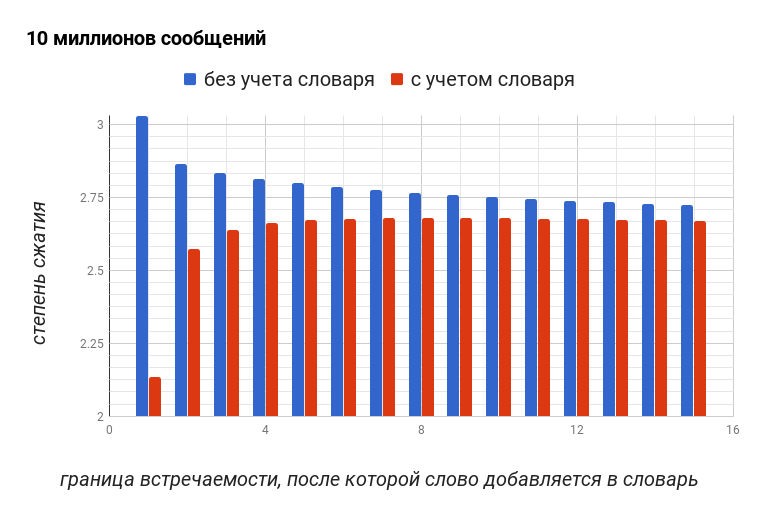
\includegraphics[width=5in]{pics/compress10m.png}
  \caption{Степень сжатия в зависимости от размера словаря (10 миллионов сообщений)}
  \label{fig2}
\end{figure}

\begin{figure}[h!]
  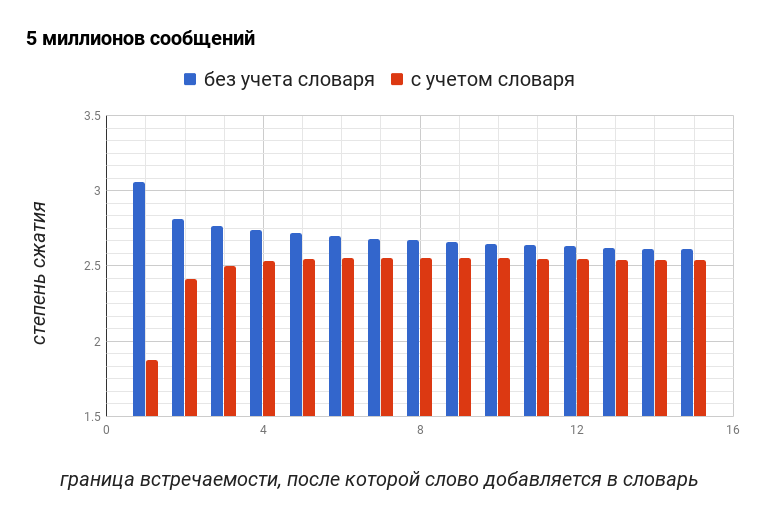
\includegraphics[width=5in]{pics/compress5m.png}
  \caption{Степень сжатия в зависимости от размера словаря (5 миллионов сообщений)}
  \label{fig3}
\end{figure}

\begin{figure}[h!]
  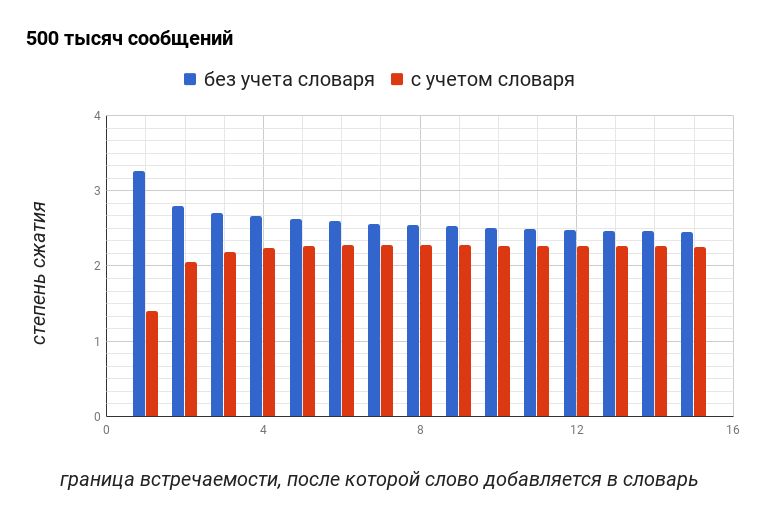
\includegraphics[width=5in]{pics/compress500k.png}
  \caption{Степень сжатия в зависимости от размера словаря (500 тысяч сообщений)}
  \label{fig4}
\end{figure}

Также интересной статистикой является размер словаря, который получается при выборе различных $K$. 
График зависимости количества слов в словаре от того, начиная с какой частоты их добавлять в словарь,
 изображен на рис.~\ref{fig5}. Аналогичный график с размером словаря изображен на рис.~\ref{fig6}. 

\begin{figure}[h!]
  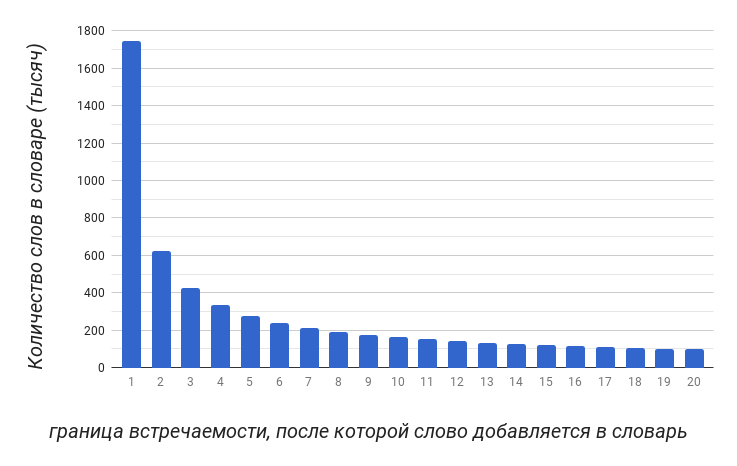
\includegraphics[width=5in]{pics/words_in_dict.png}
  \caption{Количество слов в словаре в зависимости от K}
  \label{fig5}
\end{figure}

\begin{figure}[h!]
  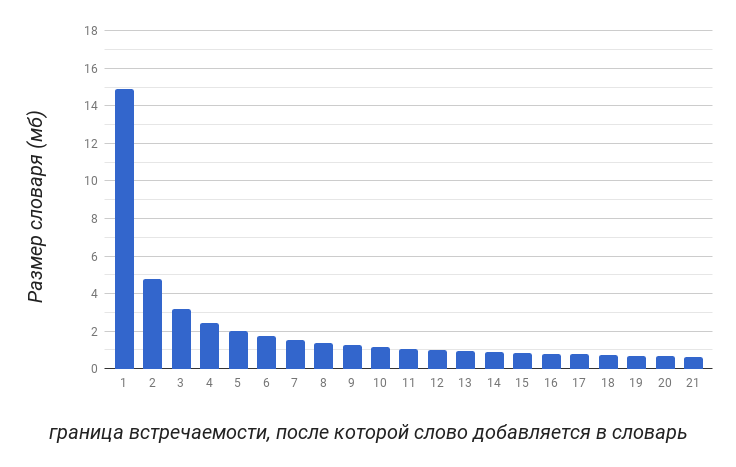
\includegraphics[width=5in]{pics/dict_size.png}
  \caption{Размер словаря в зависимости от K}
  \label{fig6}
\end{figure}

\section{Кодирование слов, которые не попали в словарь}

Описание алгоритма Хаффмана, который оперирует словами, встречается в небольшом количестве источников и во 
всех из них предлагается записывать слова, которые не встретились в словаре, как несжатую последовательность 
байт, предварительно написав символ-исключение. Такой подход разумен в случае, если в словарь добавляются все 
слова, которые встретились в тексте. Однако в нашем подходе для уменьшения размера словаря большое количество
слов исключается из него. Поэтому предлагается сжимать слова не из словаря с помощью какого-нибудь 
другого алгоритма сжатия.

Однако выбор алгоритма для сжатия таких слов не очень прост. Во-первых, алгоритм не должен использовать дополнительную память
или использовать ее мало. Во-вторых, данные для сжатия довольно плохо могут быть сжаты по своей сути. 
Например, мы знаем, что там нет слов, которые встречаются много раз. В-третьих, мы хотим
сжимать отдельные слова, а не связный текст.

Заметим, что обойтись без дополнительной памяти совсем скорее всего не получится, т. к. в отдельном сообщении максимум несколько слов,
которые не попали в словарь, и найти какие-то закономерности алгоритм не успеет.

Достаточно хорошо под критерии подходит обычный алгоритм Хаффмана, который работает с символами. 
Действительно, как было показано ранее, он использует всего один килобайт дополнительной памяти, что очень хорошо нам подходит.
Использование этого алгоритма позволило улучшить коэффициент сжатия с 2,04 до 2,38 на тестовых данных.

\section{Двухсимвольный Хаффман}

Нам хотелось еще больше соптимизировать часть сжатия, которая касается слов, которые не попали в словарь. Для этого был придуман
следующий алгоритм, который основан на обычном алгоритме Хаффмана. 

Большинство алгоритмов сжатия используют контекст, т. е. информацию о том, какие символы были закодированы последними. 
Предлагается сделать тоже самое для алгоритма Хаффмана. А именно, посчитаем $p_{ij}$~---вероятность того, что после буквы $i$ идет буква $j$.
Пусть размер алфавита равен $n$, тогда для каждого символа $i$ построим дерево Хаффмана с $n$ листьями на вероятностях $p_{ij}$. Путь в дереве $i$
до листа $j$ сопоставим строке $s_{ij}$. Алгоритм кодирования данных показан в листинге~\ref{lst1}, а декодирования в листинге~\ref{lst2}.
\begin{algorithm}[!h]
\caption{Кодирование двухсимвольным Хаффманом}\label{lst1}
\begin{algorithmic}
	\Function{Code}{$word$, $s_{ij}$}
		\State $prev \gets 0$
		\State $res \gets \text{empty string}$
		\For{$i\gets 1, len(word)$}
			\State $res \gets res + s_{prev, word[i]}$
			\State $prev \gets word[i]$
		\EndFor
		\State\Return $res$
	\EndFunction
\end{algorithmic}
\end{algorithm}

\begin{algorithm}[!h]
\caption{Декодирование двухсимвольным Хаффманом}\label{lst2}
\begin{algorithmic}
	\Function{Decode}{$encoded$, $s_{ij}, n$}
		\State $it \gets 1$
		\State $res \gets \text{empty string}$
		\State $prev \gets 0$
		\While{$it\le len(encoded)$}
			\For{$i\gets 1, n$}
				\State $len \gets |s_{prev, i}|$
				\If{$encoded[it..it + len - 1] = s_{prev, i}$}
					\State $it\gets it+len$
					\State $res \gets res + i$
					\State $prev \gets i$
					\State \textbf{break}
				\EndIf
			\EndFor
		\EndWhile
		\State\Return $res$
	\EndFunction
\end{algorithmic}
\end{algorithm}

Если при определении, какие слова нужно оставлять в словаре, суммарный размер сообщений почти не играл роли, то на коэффициент сжатия 
он влияет довольно сильно. Это происходит потому что дополнительная информация, необходимая для работы алгоритма, константного размера ($4 \cdot 256 \cdot 256 = 256 \text{ кб}$),
а значит ее относительный размер уменьшается. На рис.~\ref{fig7} показано сравнение коэффициентов сжатия следующих алгоритмов
в зависимости от количества сообщений:
\begin{enumerate}
	\item алгоритм Хаффмана по словам;
	\item алгоритм Хаффмана по словам. Слова, которые не попали в словарь, сжимаются односимвольным Хаффманом;
	\item алгоритм Хаффмана по словам. Слова, которые не попали в словарь, сжимаются двухсимвольным Хаффманом.
\end{enumerate}

\begin{figure}[h!]
  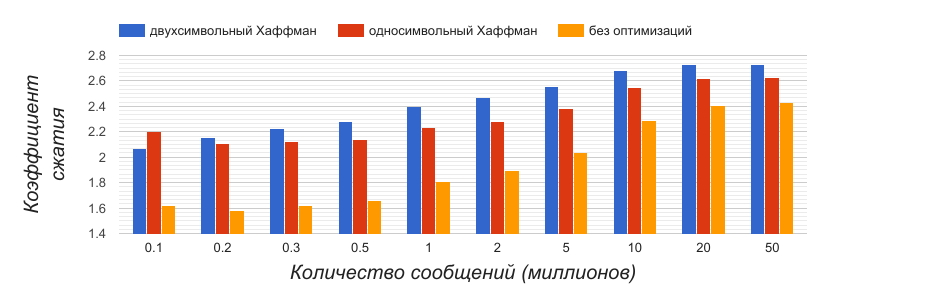
\includegraphics[width=\linewidth]{pics/compare.png}
  \caption{Коэффициент сжатия в зависимости от количества сообщений}
  \label{fig7}
\end{figure}

\section{Реализация алгоритма}

Теперь остановимся более подробно на реализации разработанного алгоритма. Наш алгоритм должен уметь выполнять следующие функции:
\begin{enumerate}
	\item train(String s)~--- использовать сообщение для тренировки;
	\item trainEnd()~--- обучение закончено. Алгоритм должен построить все необходимые ему структуры;
	\item compress(String s)~--- сжать строку. Алгоритм должен вернуть некоторую последовательность байт;
	\item decompress(byte[] data)~--- разжать строку. Алгоритм должен разжать переданные ему данные.
\end{enumerate}

Самое главное свойство алгоритма~--- для любой строки $s$ decompress(compress($s$)) = $s$.

Реализация функций train и compress во многом совпадает. Необходимо разбить исходную строку на составные части, а потом что-то с ними сделать.
Реализация функции split, которая разбивает сообщение на слова, приведена в листинге~\ref{lst3}. Он предполагает, что в коде есть функция $isAlphabetic$, которая отвечает на вопрос о том, 
как делить все символы на два различных множества. В ней нужно учесть кодировку, в которой хранятся данные, а также язык, на котором 
посылаются сообщения. Например во <<В Контакте>> есть много сообщений на украинском языке и необходимо добавить букву `i' в правильное множество.

\begin{algorithm}[!h]
\caption{Алгоритм разбития сообщения на слова}\label{lst3}
\begin{lstlisting}
 public void split(String s) {
 	boolean needAlphabetic = true;
 	for (int i = 0; i < s.length(); ) {
 		int j;
 		while (j != s.length() && isAlphabetic(s.chatAt(j)) == needAlphabetic) {
 			j++;
 		}
 		// do smth with s[i..j]
 		i = j;
 		needAlphabetic = !needAlphabetic;
 	}
}
\end{lstlisting}
\end{algorithm}

Таким образом функция train должна выглядеть также как и split, а внутри добавить слово в словарь, который соответствует $needAlphabetic$.

Функция trainEnd должна выполнить два одинаковых действия с двумя словарями. А именно из него необходимо удалить слова, которые встречаются мало раз.
При этом посчитаем вероятности $p_{ij}$ того, что после символа $i$ следует символ $j$ в этих словах. Кроме того посчитаем суммарную вероятность слов,
которые были удалены, и добавим слово-исключение с такой вероятностью.

Далее построим дерево Хаффмана для оставшихся слов. Кроме того необходимо построить $n$ дополнительных деревьев Хаффмана, где $n$~--- размер алфавита. 
$i$-е такое дерево должно соответствовать символу, который хотим написать после символа $i$. Также необходимо сделать все вероятности ненулевыми, чтобы
иметь возможность записать даже слово, которое раньше не видели.

Также необходимо добавить все слова в хеш-таблицу, в которой по слову можно узнать какое битовое представление ему соответствует.

Теперь рассмотрим реализацию функции compress. Во-первых необходимо аналогично функции split разбить сообщение на слова. Каждое слово необходимо
попытаться найти в хеш-таблице, которая соответствует $needAlphabetic$. Если слово найдено, то запишем его битовую запись и перейдем к следующему слову.
В противном случае необходимо написать слово-исключение, а потом закодировать слово с помощью двухсимвольного Хаффмана, который был описан в листинге~\ref{lst1}.

Функция decompress чуть более сложна в реализации. Она представлена в листинге~\ref{lst4}. Чтобы код не получился слишком громоздким и нечитабельным
были сделаны некоторые допущения:
\begin{enumerate}
	\item существует класс BitStream, который переводит набор байтов в последовательность битов.
	Также он умеет спускаться по переданному ему дереву Хаффмана, читая биты, и вернуть полученный лист дерева;
	\item можно пренебречь тем, что конкатенация строк работает в худшем случае за квадрат от суммарной длины.
	В реальности необходимо использовать StringBuilder;
	\item decodeTwoSybolHuffman~--- функция описанная в листинге~\ref{lst2}. 
	Можно считать, что декодирование происходит до тех пор пока не встречен специальный символ окончания.
\end{enumerate}

\begin{algorithm}[!h]
\caption{Алгоритм декодирования сообщения}\label{lst4}
\begin{lstlisting}
public String decompress(bytes[] data) {
 	String res = "";
 	BitStream bitStream = new BitStream(data);
 	boolean needAlphabetic = true;
 	while (bitStream.hasMoreData()) {
 		Token token = bitStram.readToken(needAlphabetic ? wordsTree : notWordsTree);
 		if (token.isEscapeWord()) {
 			res += decodeTwoSymbolHuffman(bitStream);
 		} else {
 			res += token.getWord();
 		}
 		needAlphabetic = !needAlphabetic;
 	}
 	return res;
}
\end{lstlisting}
\end{algorithm}

\section{Оптимизации}

На практике при реализации описанного алгоритма были применены некоторые оптимизации, 
которые позволили увеличить скорость работы алгоритма.

Рассмотрим функцию BitStream.readToken, которая была использована в листинге~\ref{lst4}. Ее реализация представлена в листинге~\ref{lst5}.
\begin{algorithm}[!h]
\caption{Спуск по дереву Хаффмана}\label{lst5}
\begin{lstlisting}
public Token readToken(TreeNode node) {
 	while (node.left != null) {
 		if (readBit()) {
 			node = node.right;
 		} else {
 			node = node.left;
 		}
 	}
 	return node.getToken();
}
\end{lstlisting}
\end{algorithm}

Такая реализация работает очень долго. У нее есть несколько проблем. 

Во-первых, на каждый бит сжатых данных происходит условный переход. 
Причем процессор не может предсказать в какую именно ветку условия нужно пойти, поскольку переходы по ним происходят примерно одинаково часто 
(за счет того, что это дерево Хаффмана). Это полностью ломает конвейерную обработку запросов процессором, что может ухудшить время работы в
несколько раз.

Во-вторых, на каждый бит сжатых данных происходит переход в случайную ячейку памяти. Поскольку размер деревьев в нашем алгоритме может 
достигать миллиона элементов, такой переход не попадет ни в какой кеш процессора.

Чтобы ускорить время выполнения этой функции была реализована следующая идея. Предподсчитаем, что сделает функция readToken, в зависимости
от того, какие будут результаты выполнения следующих 16 вызовов функции readBit для всех возможных $2^{16}$ вариантов. Существует два варианта:
\begin{enumerate}
	\item функция прочитает не более 16 бит, дойдет до листа в дереве Хаффмана и вернет его;
	\item функция прочитает все 16 бит и остановится в некоторой внутренней вершине дерева.
\end{enumerate}

Также необходимо, чтобы BitStream мог наперед выдать следующие 16 бит сжатых данных. Тогда вместо вызова readToken можно посмотреть в
предподсчитанную таблицу. После этого, если нужно, дочитать оставшиеся биты старым способом. Потом информировать BitStream 
сколько бит действительно было прочитано и вернуть нужный лист дерева.

Такой метод требует дополнительно сотни килобайт памяти, но увеличивает скорость работы в несколько раз.

Аналогично для 256 деревьев двухсимвольного Хаффмана были построены таблицы с предподсчитанными переходами на 8 бит вперед.

Кроме того важно правильно реализовать класс BitStream. В нем необходимо избегать условных переходов везде где только можно.

\chapterconclusion

В данной главе был описан разработанный алгоритм сжатия сообщений, который основан на алгоритме Хаффмана. Был детально рассмотрен вопрос размера словаря,
который необходимо использовать, а также способы кодирования слов, которые не попали в словарь. Были описаны детали реализации алгоритма, 
которые помогают увеличить скорость его работы.